\chapter{Motivation}

Advances in drone technology in recent years
have opened the door to many civilian application possibilities,
especially in the commercial sector \cite{MunichRE}.
Drones have already become today's standard in 
aerial inspection services
\cite{McKinsey, Equinox, Percepto}.
In the near future, the areas of
infrastructure,
transport,
insurance,
media and entertainment,
telecommunication,
agriculture,
safety
and mining 
are considered to be particularly promising \cite{PwC2016}.
In contrast, 
real breakthroughs of more visionary applications, 
such as drone delivery or drone taxis
are, if at all, only expected in the more distant future \cite{Rosen2019}.
Decisive reasons for this are of a technical nature. 
In particular, autonomous navigation methods are not yet 
robust enough for the reliable deployment in densely populated urban areas \cite{loquercio2018learning}.
%Considering drone delivery, 
%corporations as well as start-ups across the globe
%are conducting research. 
%Several test projects in sparsely populated areas have been realized \cite{Garcia2019}.
This master's thesis is intended to make a contribution here
by conducting basic research on integrating temporal comprehension with a recurrent convolutional neural network into
an autonomous navigation method in the closed test environment of drone racing.


In science as well as in this thesis proposal, the colloquial term "drone" refers
to the aircraft class of unmanned aerial vehicles (UAV).
The International Civil Aviation Organization (ICAO) \cite{ICAO2005} defines UAVs
as aircrafts without a human pilot onboard, 
which are either remote-controlled by a human operator or "preprogrammed and fully autonomous".
An UAV is a component of an unmanned aerial system (UAS), which additionally consist of a ground control station, communication link and payload. 
Basic components of UAVs are an airframe, an electric power system, a flight
control system and an air data terminal \cite{Fahlstrom2012}.
For UAVs with autonomous functions, additional onboard computers
provide the required computation power.
Various systems exist to classify UAVs either by 
airframe type \cite{Austin2011} or by flight key characterstics \cite{USDOD2011, Wei2016}.
With respect to the latter, 
Watts, Ambrosia and Hinkley \cite{Watts2012} proposed a classification system 
for scientific usage.
Table \ref{tab:UAV_classification_system_by_Watts_Ambrosia_and_Hinkley} shows a selection of the system's UAV sub-classes.
My master's thesis is primarly associated with quadcopters,
the MAV representatives that, according to my observations,
prevail among private, scientific and commercial applications as the "typical" drone model.


%UAVs originate from the military, were adopted by
%enthusiasts, have gained more and more acceptance in the industry and finally have become today's standard in 
%aerial inspection services in
%agriculture,
%construction,
%infrastructure,
%utilities,
%and mining \cite{McKinsey, Equinox, Percepto}.
MAVs exhibit several substantial advantages over ground vehicles due to their aerial maneuverability and agility.
As they are unaffected by many obstacles and largely independent of infrastructure,
destinations can be reached by the shortest route, waiting times can be avoided
and the effort and risk of getting to places that are difficult to access can be reduced \cite{Watts2012}.
In addition, from the privileged perspective of a bird, onboard sensors 
are able to record extensive data of high quality fast at low costs
which is extremly valuable in the present context of big data and machine learning \cite{PwC2016, Garcia2019}.
On the downside,
MAVs, as small aircraft vehicles, can move substantially less weight, 
whereby, computational power, mission-specific payload and battery capacity is severely limited.
Limited battery capacity, in turn, restricts flight range and duration.
Therefore, for MAVs paying off economically, efficiency is paramount.
A central approach to increase efficiency is to shift functions from a human operator to the drone itself,
i.e., increase the drone's degree of autonomy.
This becomes particularly clear in the example of delivery applications.
Because MAVs can load significantly fewer packages and
have to recharge more often than conventional delivery trucks have to refuel,
one human pilot per drone would be too ineffective for a broad deployment.
Drone delivery systems are only profitable
if most functions are performed autonomously by the individual delivery drone,
or, at best, by the collective of the drone swarm \cite{Chiang2019, Lee2017}.
So far, MAVs have proven their commercial value in fields associated with large industrial sites
which usually provide flight environments that are essentially demarcated and controlled.
State-of-the-art autonomous drones are capable of dealing with these highly predictable environments.
Here, mention can be made of drone-in-a-box systems:
the box provides takeoff/landing and charging infrastructure for
the drone or drone swarm, that autonomously execute preprogrammed flight missions \cite{drones5040108}.
In contrast, the open-world environments of our daily lives 
are densely disturbed and are, thus, characterized by high uncertainty.
The resulting technical complexity, 
notably with respect to "navigation, communication and automatization" \cite{kellermann2020drones},
is a major cause that
autonomous drones have not yet asserted themselves for commercial applications in those environments.
Other main reasons are legal restrictions and lack of acceptance \cite{Rosen2019}.


Autonomous navigation is a highly relevant topic in current UAV-related public research.
State-of-the-art autonomous navigation methods 
lack in robustness to safely exhaust the full agility of UAVs in complex environments \cite{loquercio2018learning}.
Navigation, as an integral functionality,
comprises the main task of achieving a desired pose or position
while performing necessary sub-tasks at the same time \cite{loquercio2018learning}.
The complexity of the flight environment
determines the necessity of individual sub-tasks 
and, thus, the complexity of the navigation method.
In controlled airspace 
navigating through pre-planned waypoints only relying on global navigation satellite system (GNSS) 
sensors may be sufficient.
In uncontrolled airspace sub-tasks 
such as obstacle avoidance and the coordination with other agents are required.
Under the assumption that temporal comprehension is a strong measure
to increase robustness in autonomous navigation,
this thesis intends to explore the effect of using a recurrent convolutional neural network in the environment of drone racing.
The drone racing environment provides simplified test conditions, where a mere 
reactive control from race gate to race gate is sufficient,
and is therefore very convenient for this basic research.





%Consequently, 
%whether the state of the art in autonomous navigation of UAVs
%is sufficiently robust depends on the flight environment and the flight mission.
%Again, drone delivery provides an explanatory example here.
%Projects have been already 
%realized in rural areas where the airspace is mainly undisturbed [].
%Here, navigating through waypoints only relying on GNSS 
%without any implementation of obstacle avoidance and agent-coordination may be sufficient. 
%In contrast, urban areas are full of unstructered obstacles and other participating agents 
%which result in a high uncertainty that cannot be faced with in-advance planning. 
%Only a high level of autonomy in navigation
%could robustly cope with the challenges of this environment.
%This level has not yet been achieved.


%Research on autonomous MAV navigation mainly relies on deep learning 
%which allows to comprehend the immediate environment based on the perception of
%onboard sensors. \cite{loquercio2018learning}
%State-of-the-art navigation methods 
%achieve a high spatial understanding of the environment
%by feeding convolutional neural networks with RGB or depth data.
%This research aims to develop a simple navigation method 
%that extend this spatial perception onto temporal extension 
%by serially connecting a CNN with a long-short-term-memory (LSTM) network.
%Based on my assumption that powers of recall are crucial for humans when navigating,
%I am convinced that future autonomous navigation systems will also encompass this ability.
%The navigation method will be tested in simulation and real world in a simplified test scenario,
%which, however, requires the MAV to remember the expansion and relative motion of obstacles while considering its own elapsed acceleration.




\chapter{Objectives}\label{cha:objectives}
%Public research has put forth many advanced methods for autonomous navigation of MAVs.
%However, they are not sophisticated enough to conquer open-world environments of high uncertainty
%such as urban areas \cite{loquercio2018learning}.
%In current research, deep learning techniques that empower MAVs with comprehension abilities
%constitute the best approach to face the uncertainty of these environments.
%State-of-the-art navigation methods 
%integrate feedforward, deep convolutional neural networks
%that map the current color or depth image to action.
%Thereby a high, spatial comprehension
%of the immediate surrounding of the MAV can be achieved.
%But I suspect that the mere understanding of space, as sophisticated as it may be,
%is not sufficient for robust autonomous navigation of MAVs in open-world environments.
%Therefore, I aim to develop a navigation method 
%that besides spatial also includes temporal comprehension.

Many advanced methods for autonomous navigation of MAVs
integrate feedforward, deep convolutional neural networks (CNN)
that, with a high spatial comprehension of the MAV's immediate surrounding, 
map the current color or depth image to prediction or action.
With my thesis I aim to develop a navigation method for the drone racing environment
using a recurrent convolutional neural network (R-CNN)
that, due to its recurrency, can not only spatially but also temporally comprehend.
I would like to examine if infering navigation decisions from present and \textbf{past} sensor data
is beneficial to the robustness at high speeds and can cope with the event of intermediate target loss (see below).
%The following objectives should be achieved within the scope of the master's thesis.

The baseline of my thesis is a vision-based navigation method for drone racing
developed by Kaufmann et al. from ETH Zurich in 2018 \cite{Kaufmann2018},
that stood out with high reliability and agility on high speed, dynamic flight curves.
The method is hybrid, i.e., 
it consists of a convolutional neural network (CNN)
serially connected to a conventional control system
At a frequency of 50 Hz, the following steps are repeatedly executed:
\begin{itemize}
	\item[1.] Input the current raw 300x200 RGB image from the onboard, forward-facing camera to the CNN.
	\item[2.] The CNN predicts a waypoint in the 2D reference frame of the image and a normalized speed:
				$x_\text{IRF}, y_\text{IRF} \in [-1, 1],\ v_\text{NORM} \in [0, 1]$ 
	\item[3.] Transform the waypoint from the image reference frame to the reference frame of the autopilot state estimation: 
				$x_\text{ARF}, y_\text{ARF}, z_\text{ARF} \in \mathbb R^3$.
	\item[4.] Compute a minimum-jerk (time derivative of acceleration) trajectory from the current autopilot state estimate to the waypoint.
				The duration of the trajectory depends on the predicted normalized speed $v_\text{NORM}$.
	\item[5.] Push the states of the trajectory to the autopilot.
	\item[6.] The autpilot, using conventional algorithms, generates control commands and triggers their execution.
				Thereby, the end state of the trajectory is never reached since the re-planning of the trajectory is continually triggered by new waypoints.
\end{itemize}
According to the paper, the baseline has a success rate of 100 \% on the simulated racetrack when 
the maximum speed is not greater than 9 m/s. For higher maximum speeds
\{10, 11, 12\} m/s the success rate decreases to approximately \{85, 60, 35\} \%.
Besides maximum speed, the simulated racetrack is designed in way that at any time the 
currently targeted race gate is located in the frame of view (FOV) of the onboard camera.
This is a requirement of the baseline because the CNN derives its navigation decisions only
from the current image. In the event of intermediate target loss, i.e.,
there is no race gate in the FOV and, consequently, on the image, the baseline 
must result in undefined behaviour. 
Intermediate target loss could for example 
happen in the case of a steep curve between two consecutive race gates
or in the case of an obstacle that temporally blocks the view to the currently targeted gate.


In my thesis I plan to further develop only the first part of the hybrid approach.
I intend to, first, replace the CNN with a R-CNN and,
second, feeding additional features, i.e., data from the inertial measurement unit (IMU), to the network.
The IMU data encompasses three (x, y, z) linear accelerations and three (x, y, z) angular velocities.
I expect that thereby, 
waypoints are not only generated on the basis of the current RGB image and IMU data, 
but that also past sensor data is included in the navigation decision.
This would possibly result in the following positive effects:
\begin{itemize}
	\item Making decisions on the basis of a series of sensor data makes the network more robust against outliers.
			Otherwise, at high speeds, outliers may directly result in a crash.
	\item Considering the similarity of recurrency to mathematical integration,
			feeding IMU data to the network could have great potential since the network could be more or less able to internally estimate positions and orientations.
	\item Due to its "memory", the network is able to generate meaningful waypoints in the case of intermediate target loss, i.e.,
			the next gate of the race track is not depicted in the current image, but has appeared in previous images.
	%\item Due to temporally distributed images, the network is able to take the speeds of moving gates (or obstacles) into the account of the navigation decisions.
	\item Because trajectories are temporally extended maneuvers, a network with temporal comprehension is more able to imitate the expert system.
			Thus, the resulting trajectory through the race track formed 
			by the successively generated waypoints 
			is more similar to a precomputed optimal trajectory.
\end{itemize}
The approach is implemented utilizing the middleware ROS \cite{ros}
and simulated with the photo-realistic Flightmare Simulator \cite{song2020flightmare} built on Unity.
For the implementation concept, see section \ref{sec:implConcept}.
In simulation, the following tests should be conducted to compare my approach to the baseline.





\paragraph{Randomized Figure-8 Drone Racing}
Conduct test runs with increasing maximum speeds.
For each run,
build a randomized figure-8 drone racing track
and test my approach and the baseline on the track.
For each maximum speed, evaluate the percentage share of successful runs,
the average time of racetrack completion
and the
closeness to the global trajectory in terms of optimality.
The latter could be computed by recording the reference states
that are continually pushed to the autopilot,
taking the 4th derivative with respect to time (snap)
and integrate the values.
The in this way calculated cost could be used to measure closeness to
the optimal, minimum snap global trajectory which the expert system used to generate the 
training data.


\paragraph{Intermediate target loss on sharp curve}
Simulate two gates with a sharp curve in between.
Before the drone passes the first gate,
both successive gates must appear in the frame of view of the onboard camera.
The curve must be so sharp, that, after traversing the first gate, not only the first but also the second gate has left the frame of view.
The baseline, whose CNN makes navigation decisions from only the current image, will likely to fail in this scenario
due to the absence of a goal.
In contrast, my approach uses an R-CNN which is able to internally store information from previous images.
In case that the R-CNN is well trained, it should be able to generate meaningful waypoints to complete the sharp curve and traverse the second gate.
This becomes especially true, if the R-CNN is able to make use of the IMU data estimating poses.
The percentage share of successful runs would be a convenient metric for evaluation.

%Tests to compare my extended approach with the original method should be designed
%and conducted to investigate if the above enhancements could be realized.



%My work is based on the paper of Kaufmann et al. \cite{Kaufmann2018} from 2018.
%Just recently, follow-up work from ETH Zurich \cite{Loquercio2021Science} with 
%a way more sophisticated autonomous navigation method has been published. 
%The neural network is designed to cover a bigger scope
%by directly outputting trajectories instead of waypoints in image coordinates.
%However, I intend to still base my work on the earlier paper,
%since the more modular design provides a very good starting point with respect to my intended basic research
%whether temporal comprehension leads to improvements in autonomous navigation.
%Moreover, the test environment of drone racing is very convenient due to its simplicity.
%The completion of the race track can be achieved by mere reactive control to the next gate
%and does not require the formulation of a high level navigation goal
%whose implementation would pose another challenge.




%- As mentioned above, the navigation method theoretically does not require a high-level goal formulation
%since the reactive targeting the next gate already results in completing the race track.
%Practically, in the event that at any time the next gate is not located 
%in the frame of view (FOV) of the MAV's onboard camera,
%the output of the deep neural network (DNN) is not defined and the lack of a high-level goal becomes evident.
%This is also the case, even if the MAV has seen the next gate in the past (see figure ??).

%- In addition, humans cannot estimate the velocity and direction of motion of themselves, obstacles or other agents
%based on a short blink with their eyes but they need to observe over at least a short period of time.
%- Not only localization but also situational reasoning is strengthened by memory,
%e.g., a car driver observes a child that runs from the sidewalk through the parking cars onto the road
%and has enough reaction time or even anticipation to brake.
%Without any power of recall, the driver may start braking in anticipation
%when the child is still on the sidewalk, but may stop braking after the child disappears behind a parking car.
%
%- dynamic trajs

%In the navigation method of this research, I want to meet the lack of high-level goal planning 
%by introducing powers of recall to navigation.
%To my knowledge, Kelchtermans and Tuytelaars \cite{Kelchtermans2017}
%are the only ones who used a recurrent neural network for memory abilities in autonomous, 
%vision-based UAV navigation. \cite{Shakeri2019}
%-reason why their work is not what i want..
%However, they only tested their method in simulation and did not comprehensively evaluate their results.
%If the method, after passing the first gate, could remember that it has seen the second gate before,
%the method could plan to navigate through the second gate based on elapsed images.

%In my method, I plan to use a LSTM-CNN which is a deep convolutional neural network
%serially connected to a long-short-term-memory (LSTM) neural network.
%
%While the CNN has the ability to perceive and reason spatial structures of the immediate environment,
%the LSTM is able to establish connections through time. 
%
%In other words, the CNN is responsible to predict waypoints 
%or generate trajectories based on single images,
%whereas the LSTM empower the method to recall and remember 
%by evaluating the temporal structure between the predictions of the CNN.
%
%Besides the above steep curve scenario, this memory would show great benefit in situations
%when the quadcopter lost track of the goals and it can recall elapsed images.
%In case of the application in urban areas, for example, 
%quadcopters could remember obstacles 
%that were visible but have become occluded and thus, could better anticipate. 
%Or after an evasive maneuver, 
%the quadcopter could return to the actual path 
%much faster because he memorizes its maneuver.
%In that sense, the memory of the quadcopter is another form of localization in the environment, 
%which is not global but namely local.
%In addition, memory could enable better optimization, e.g., 
%the imitation learning of optimal trajectories which
%are not only spatial but also temporal objects.
%However, this research, in a simplified scenario, should only prove if powers of recall 
%are applicable and generally useful for the autonomous navigation of MAVs.

\chapter{Task Packages}
Based on the objectives, the following task packages are defined:

\begin{itemize}
	\item Build the drone racing simulation.
	\begin{itemize}
		\item[{[}X{]}] Familiarize with Flightmare \cite{song2020flightmare}, a photo-realistic simulator for quadcopters.
		\item[{[}X{]}] Familiarize with the Unity Engine \cite{Unity}, to create and manipulate the rendered environments in Flightmare.
		\item[{[}X{]}] Transfer the already implemented simulation from Gazebo \cite{Koenig2004} to Flightmare. For exemplary training data generated in Gazebo see section \ref{sec:GazeboTrainingData}.
	\end{itemize}
	\item Generate training data in simulation.
	\begin{itemize}
		\item[{[}X{]}] Adjust the already implemented expert system (see section \ref{sec:expert_system}), so that the training data includes
		an RGB image and IMU data of the drone as features and a waypoint and desired speed as labels.
		\item[{[}X{]}] Run simulation to generate the data.
	\end{itemize}
	\item Build the recurrent convolutional neural network (R-CNN).
	\begin{itemize}
		\item Familiarize with PyTorch \cite{NEURIPS2019_9015}.
		\item Transfer already implemented data input pipeline from TensorFlow \cite{tensorflow2015-whitepaper} to PyTorch.
		\item Familiarize with R-CNNs.
		\item Design the R-CNN using hyperparameters for later adjustments.
		\item Implement the R-CNN in PyTorch.
		\item Train the R-CNN and find best values for the hyperparameters. Use mean squared error as metrics for regression.
	\end{itemize}
	\item Evaluate my approach.
	\begin{itemize}
		\item Design test scenarios (see section for comparison with the base navigation method of Kaufmann et al. \cite{Kaufmann2018}.
		\item Implement and conduct tests in simulation. 
		\item Evaluate results of tests.
	\end{itemize}
	\item Write thesis documentation.
	\item (Optional) Conduct test in real world.
	\begin{itemize}
		\item Implement my approach on real drone.
		\item Find test site and rebuild a test scenario that in simulation produced promising results.
		\item Conduct test, evaluate and document in thesis.
	\end{itemize} 
 
\end{itemize}

	
\chapter{Time Schedule}

\begin{figure}[H]
    \centering
    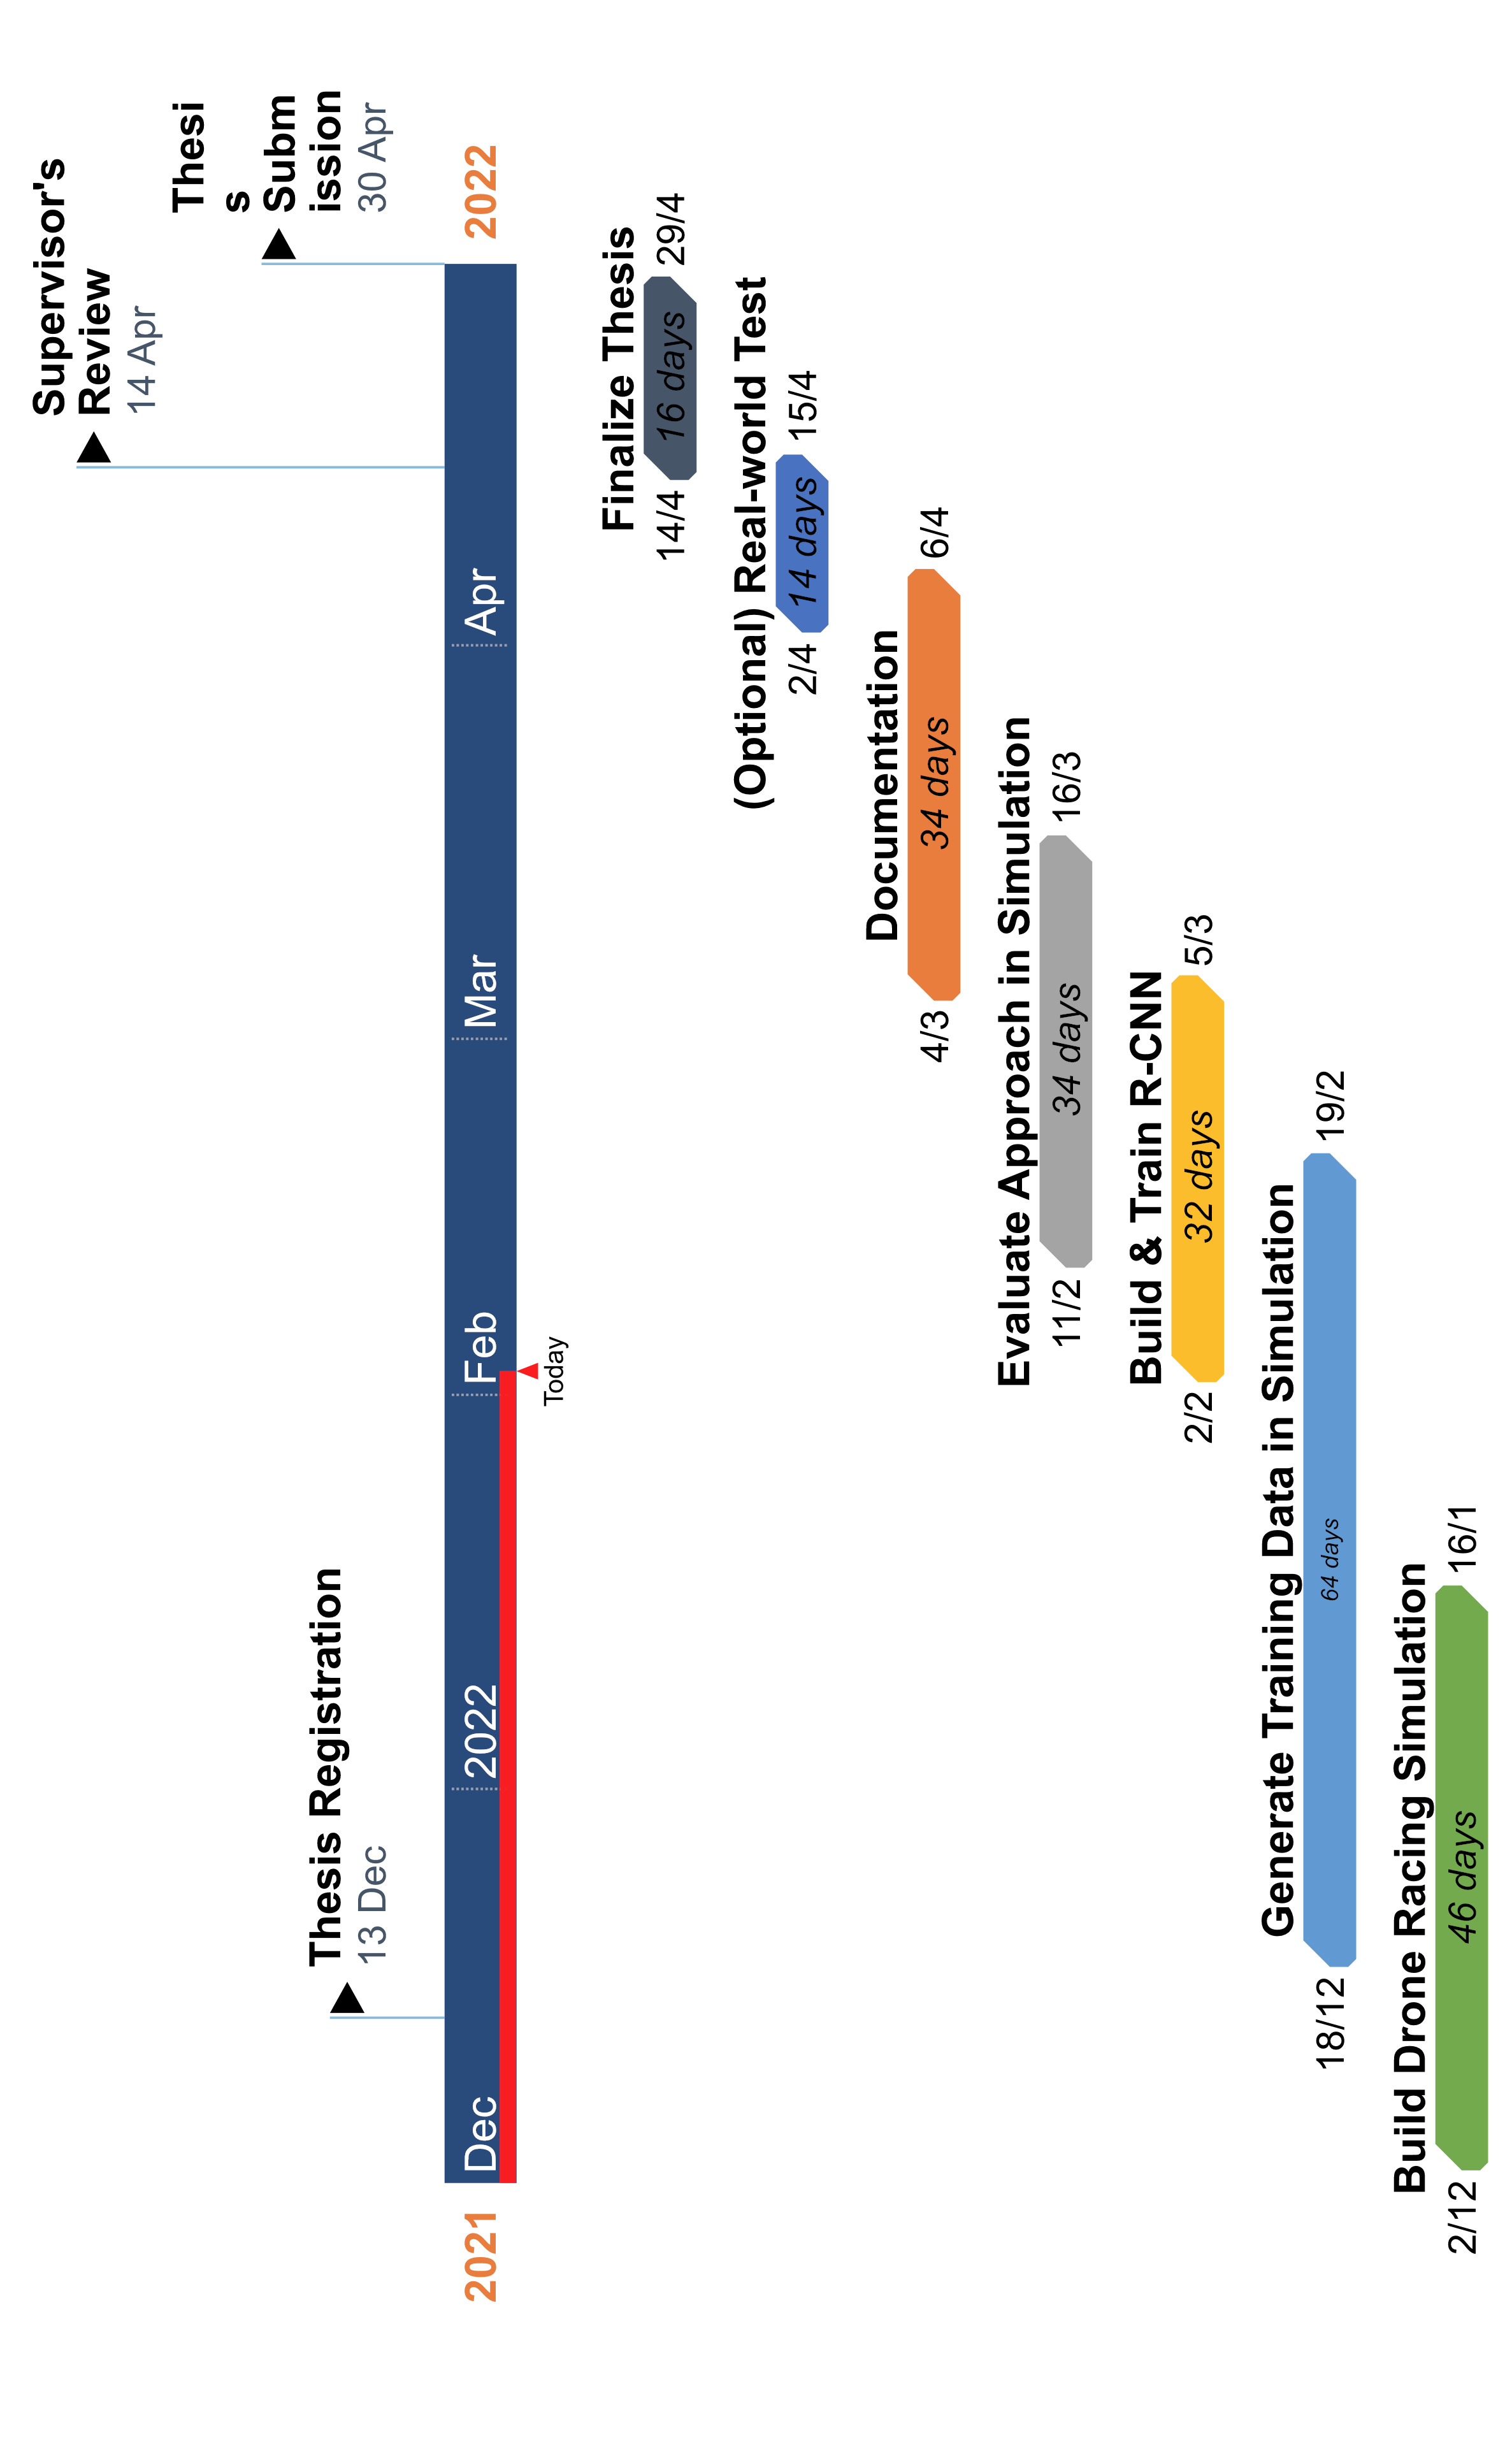
\includegraphics[width=0.6\textwidth]{figures/Software Development.png}
%    \decoRule
    \caption[Gannt diagram illustrating the time schedule of the master's thesis.]{Gannt diagram illustrating the time schedule of the master's thesis. \textit{Created with \href{https://online.officetimeline.com/}{Office Timeline Online}}}
    \label{fig:Timeline}
\end{figure}

\chapter{Organizational Matters}
\begin{itemize}
	\item Language of the thesis: English
	\item Text processing system: LaTeX
	\item Programming languages: C++, Python
	\item Supervisor: Dr. rer. nat. Yuan Xu
	\item Reviewers: Prof. Dr. Sahin Albayrak, Dr.- Ing. Stefan Fricke
\end{itemize}

\chapter{Annex}


\section{Selected UAV Classes of the Classification System by Watts, Ambrosia and Hinkley}
\begin{table}[H]
    \caption[Selected UAV Classes of the Classification System by Watts, Ambrosia and Hinkley]
	{Selected UAV Classes of the Classification System by Watts, Ambrosia and Hinkley: 
	micro air vehicles (MAV), low altitude short endurance (LASE), 
	low altitude long endurance (LALE), medium altitude long endurance (MALE) and 
	high altitude long endurance (HALE). \textit{Compiled from \cite{Watts2012}.}}
    \label{tab:UAV_classification_system_by_Watts_Ambrosia_and_Hinkley}
    \centering
    \begin{tabular}{r l l l L{0.3\textwidth}}
    \toprule
    \tabhead{Class} & \tabhead{Altitude} & \tabhead{Endurance} & \tabhead{Range} & \tabhead{Takeoff/Landing} \\
    \midrule
    MAV     & < 330 m       & < 30 min  & < 1 km        & Any small area \\
    LASE    & < 450 m       & < 2 h     & < 10 km       & Human hand, catapult system or runway \\
    LALE    & < 5,000 m     & < 20 h    & < 100 km      & Runway \\
    MALE    & < 9,000 m     & < 40 h    & < 1,000 km    & Runway \\
    HALE    & < 25,000 m    & < 30 h    & < 10,000 km   & Runway \\
    \bottomrule\\
    \end{tabular}
\end{table}

%\section{Steep curve scenario}
%
%For example, a section of the racetrack that consist of two successive gates, in between a steep curve
%could not successfully be navigated through by the method, even if both gates have already appeared on images.
%Before the MAV navigate through the first gate, both gates are in the FOV of the camera.
%After it has flown through the first gate, because the curve is too steep, the second gate is out the FOV 
%and the navigation method has no goal to be achieved.

% Taking a human as example
% HUMAN IN THE DRONE RACETRACK EXAMPLE
%To solve this problem I consider what a human would do in this scenario.
%From a position before entering the gate 1, a human can see gate 1 and 2.
%After he flew through gate 1, he has no visual contact to both gates anymore.
%Yet, he can manage to navigate through gate 2 because he has the ability 
%to remember the position of gate 2 in his body frame. 


\section{The Expert System}\label{sec:expert_system}

In machine learning, an expert system is a program that imitates a human expert in order to solve a problem. 
It comprises two main components: a \textit{knowledge base} that stores known facts and rules, and an
\textit{inference engine} which, by applying the rules to the known facts,
generates new facts \cite{jackson1986introduction}.

For the navigation method of my thesis, 
I have already re-implemented the expert system (in the paper, referred to as expert policy) 
by Kaufmann et al. \cite{Kaufmann2018} as a function within a ROS node. 
I extended the expert in order that it also records the IMU data as labels. 
The following structure summarizes the expert system:

\begin{itemize}
	\item Problem to solve
	\begin{itemize}
		\item Replace the yet untrained CNN when navigating the drone through the drone race track by
		generating the inputs (i.e., a waypoint in image coordinates ($x, y \in [-1, 1]$), desired speed) 
		to the conventional control system (see chapter \ref{cha:objectives}).
		\item While flying through the race track, 
		generate training data (i.e., RGB images, IMU data) 
		with labels (i.e., a waypoint in image coordinates ($x, y \in [-1, 1]$), desired speed).
	\end{itemize}
	\item Knowledge base
	\begin{itemize}
		\item Known facts
		\begin{itemize}
			\item Center points of the gates that build the drone race track.
			\item A pre-computed, minimum-snap trajectory (referred to as global trajectory) traversing the center points of the gates.
			\item Continually updated, ground-truth state of the drone.
			\item Current gate (i.e., the gate that needs to be traversed next when completing the race track) 
			and last gate (i.e., the gate that has been traversed most recently)
		\end{itemize}
		\item Rules
		\begin{itemize}
			\item Project the current drone state to a state of the global trajectory and name this state expert state. 
			For more details of the rather complex projection, see the original paper.
			\item If the drone is more distant to the expert state than a user-specified parameter, 
			set the expert state to the state of the global trajectory with minimum distance to the drone.
			\item Set the desired speed (component of the label) to the velocity of the state 
			that is ahead of the expert state with a user-specified distance. 
			However, the desired speed is bounded by a user-specified minimum and maximum speed 
			as well as a user-specified maximum speed increment with respect to the current speed of the drone.
			\item Compute the horizon (a distance) as the product of a user-specified time duration and the desired speed. 
			However, the horizon must not be greater than the distances to the current and last gate.
			\item Set the waypoint in image coordinates, $x, y \in [-1, 1]$, (component of the label) by projecting the position of the state,
			which is ahead of the expert state with a distance equal to the horizon, onto the image. 
			Do this in consideration of the current state of the drone.
		\end{itemize}
	\end{itemize} 
	\item Inference engine
	\begin{itemize}
		\item Implemented as a set of functions within a C++ ros node, that fetches the known facts via ROS topics or computes and store them as internal variables.
		\item The user can de-/activate the expert system as functional part of the navigation method.
	\end{itemize} 
\end{itemize}







\section{Labeled training data generated in simulation with Flightmare/Unity}\label{sec:GazeboTrainingData}

\begin{figure}[H]
	\centering
	\begin{subfigure}[b]{1.0\textwidth}
		\centering
		\begin{minipage}[c]{0.37\textwidth}
			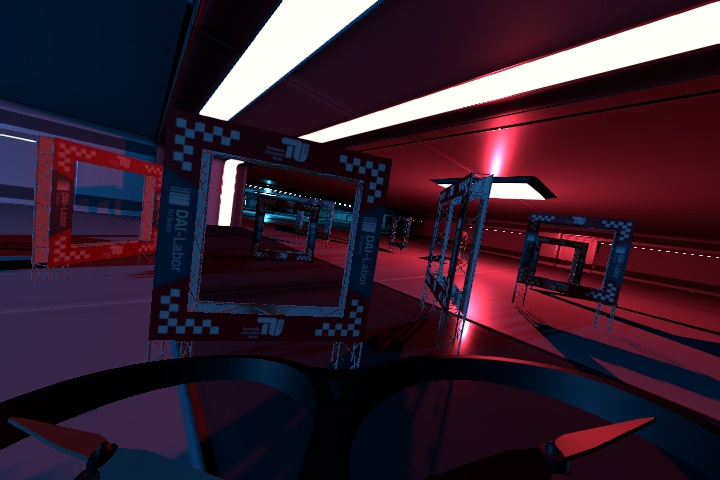
\includegraphics[width=\textwidth]{figures/camera_frame_00180.jpg}
	  	\end{minipage}\hfill
	  	\begin{minipage}[c]{0.5\textwidth}
			\caption{
				\textbf{IMU Data}\\
				$a_x = -0.731,\ a_y = -0.030,\ a_z = 9.610$\\
				$\omega_x = 0.074,\ \omega_y = -0.006,\ \omega_z = 0.479$\\
				\\
				\textbf{Labels}\\
				$x_\text{IRF} = -0.302,\ y_\text{IRF} = 0.077$\\
				$v_\text{NORM} = 0.892$
				}  
				%\label{fig:03-03}
	  	\end{minipage}
	\end{subfigure}
	\begin{subfigure}[b]{1.0\textwidth}
		\centering
		\begin{minipage}[c]{0.37\textwidth}
			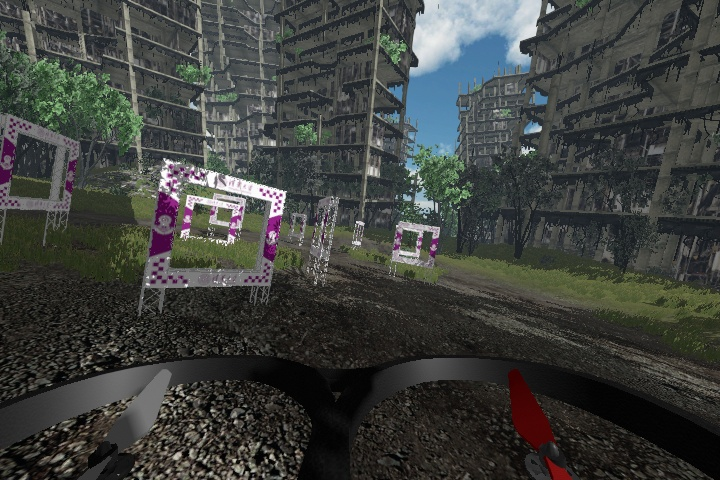
\includegraphics[width=\textwidth]{figures/camera_frame_00400.jpg}
	  	\end{minipage}\hfill
	  	\begin{minipage}[c]{0.5\textwidth}
			\caption{
				\textbf{IMU Data}\\
				$a_x = -0.650,\ a_y = -0.058,\ a_z = 9.675$\\
				$\omega_x = 0.001,\ \omega_y = 0.148,\ \omega_z = 0.519$\\
				\\
				\textbf{Labels}\\
				$x_\text{IRF} = -0.428,\ y_\text{IRF} = 0.136$\\
				$v_\text{NORM} = 0.920$
				}  
				%\label{fig:03-03}
	  	\end{minipage}
	\end{subfigure}
	\begin{subfigure}[b]{1.0\textwidth}
		\centering
		\begin{minipage}[c]{0.37\textwidth}
			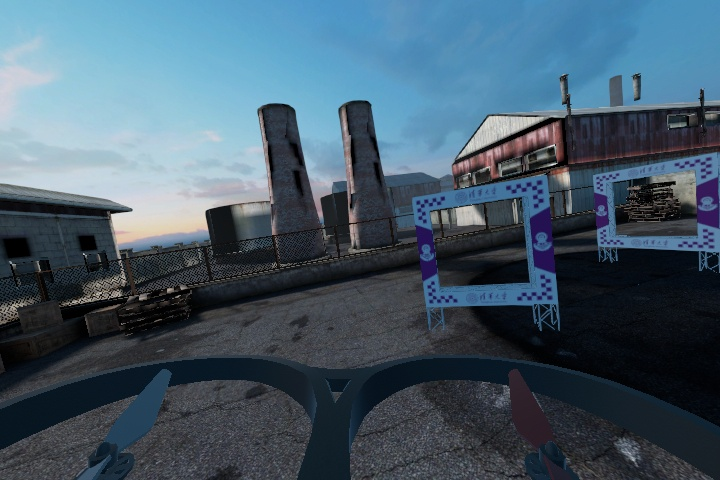
\includegraphics[width=\textwidth]{figures/camera_frame_00600.jpg}
	  	\end{minipage}\hfill
	  	\begin{minipage}[c]{0.5\textwidth}
			\caption{
				\textbf{IMU Data}\\
				$a_x -0.714= ,\ a_y = 0.059,\ a_z = 9.608$\\
				$\omega_x = 0.058,\ \omega_y = -0.153,\ \omega_z = -0.362$\\
				\\
				\textbf{Labels}\\
				$x_\text{IRF} = 0.403,\ y_\text{IRF} = -0.003$\\
				$v_\text{NORM} = 0.893$
				}  
				%\label{fig:03-03}
				%-0.714		0.059	9.608	0.058	-0.153	-0.362	%	0.403	-0.003	0.893
	  	\end{minipage}
	\end{subfigure}
	\begin{subfigure}[b]{1.0\textwidth}
		\centering
		\begin{minipage}[c]{0.37\textwidth}
			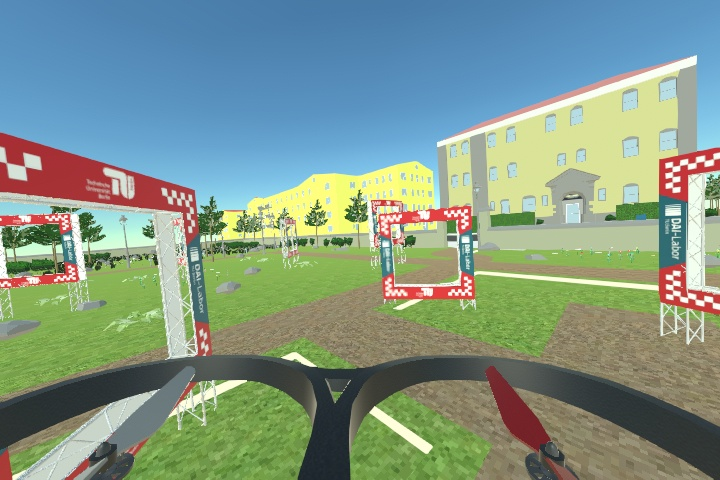
\includegraphics[width=\textwidth]{figures/camera_frame_00800.jpg}
	  	\end{minipage}\hfill
	  	\begin{minipage}[c]{0.5\textwidth}
			\caption{
				\textbf{IMU Data}\\
				$a_x = -0.625,\ a_y = 0.034,\ a_z = 9.620$\\
				$\omega_x = 0.003,\ \omega_y = -0.068,\ \omega_z = -0.207$\\
				\\
				\textbf{Labels}\\
				$x_\text{IRF} = 0.183,\ y_\text{IRF} = -0.128$\\
				$v_\text{NORM} = 0.756$
				}  
				%\label{fig:03-03}
	  	\end{minipage}
	\end{subfigure}
	\begin{subfigure}[b]{1.0\textwidth}
		\centering
		\begin{minipage}[c]{0.37\textwidth}
			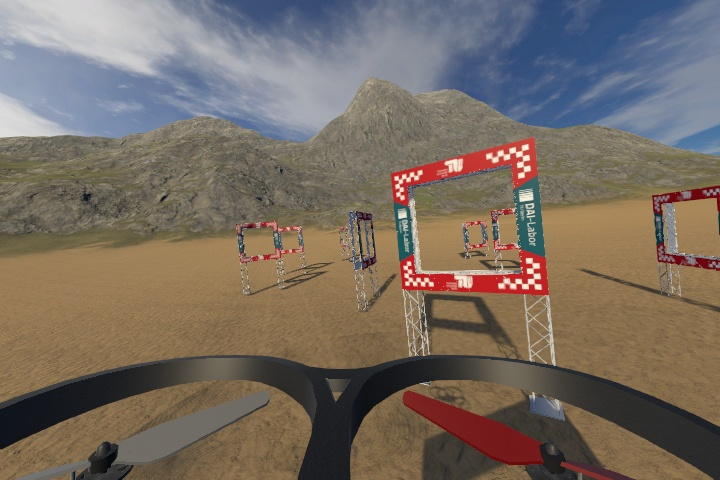
\includegraphics[width=\textwidth]{figures/camera_frame_01000.jpg}
	  	\end{minipage}\hfill
	  	\begin{minipage}[c]{0.5\textwidth}
			\caption{
				\textbf{IMU Data}\\
				$a_x = -0.648,\ a_y = 0.044,\ a_z = 9.781$\\
				$\omega_x = 0.019,\ \omega_y = 0.029,\ \omega_z = -0.295$\\
				\\
				\textbf{Labels}\\
				$x_\text{IRF} = 0.293,\ y_\text{IRF} = 0.104$\\
				$v_\text{NORM} = 0.749$
				}  
				%\label{fig:03-03}
	  	\end{minipage}
	\end{subfigure}

	\caption{Five Samples of labeled training data, generated in simulation of a randomized drone figure-8 racetrack in five different scenes with Flightmare/Unity. 
	Features: 720x480 RGB image, linear accelerations and angular velocities of IMU. Labels: x-, y-coordinate of waypoint in image reference frame, normalized speed.}
	\label{fig:three graphs}
\end{figure}



\section{Implementation Concepts}\label{sec:implConcept}


\begin{figure}[H]
    \centering
    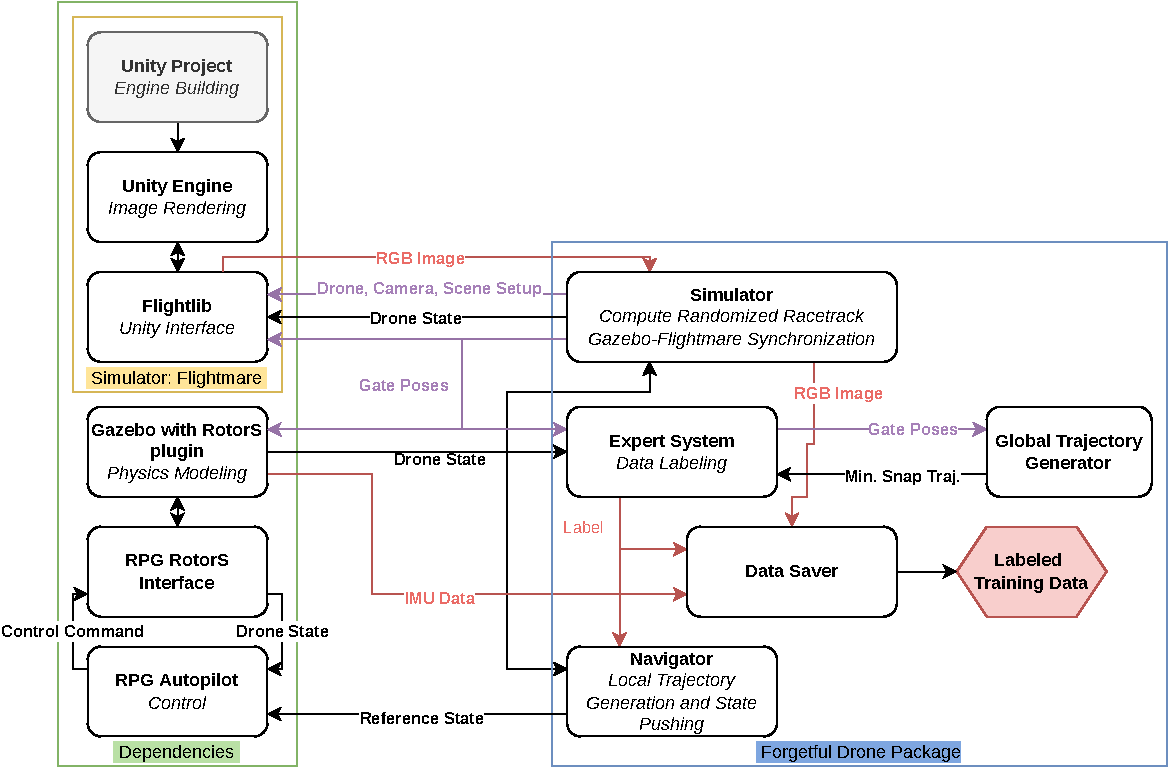
\includegraphics[width=1.0\textwidth]{figures/implementation_concept_training_data_generation.drawio.pdf}
%    \decoRule
    \caption[Implementation Concept, Training Data Generation]{\textbf{Implementation Concept, Training Data Generation:}
	The Simulator computes a drone racetrack consisting of randomized gate poses. It sends the race gate poses to Flightmare to render the gates,
	to Gazebo to model collisions and to the Expert System. The Expert System forwards the gate poses to the Global Trajectory Generator
	which computes a minimum snap trajectory and sends it back to the Expert System. Then the Simulator sets up Flightmare 
	(drone and camera configurations, scene, site and race gate type). Then a run to generate training data starts.
	The Simulator continually receives the ground truth state of the drone and sends it to Flightmare for rendering.
	Additionally, the Simulator continually receives an RGB image from Flightmare and sends it to the data saver.
	The Expert system, based on the ground truth state of the drone and the global trajectory, computes the label 
	(2D waypoint in image coordinates, normalized speed) and sends it to the Data Saver and the Navigator.
	In addition to the RGB image and the labels, the Data Saver is receiving the ground truth IMU data from Gazebo.
	The data saver saves the features (RGB image and IMU data) and the labels. 
	The Navigator, based on the labels, computes a minimum jerk local trajectory and pushes the states to the RPG Autopilot.
	The RPG Autopilot tracks the reference states receiving ground truth drone states.}
    \label{fig:OverviewDiagram}
\end{figure}

\begin{figure}[H]
    \centering
    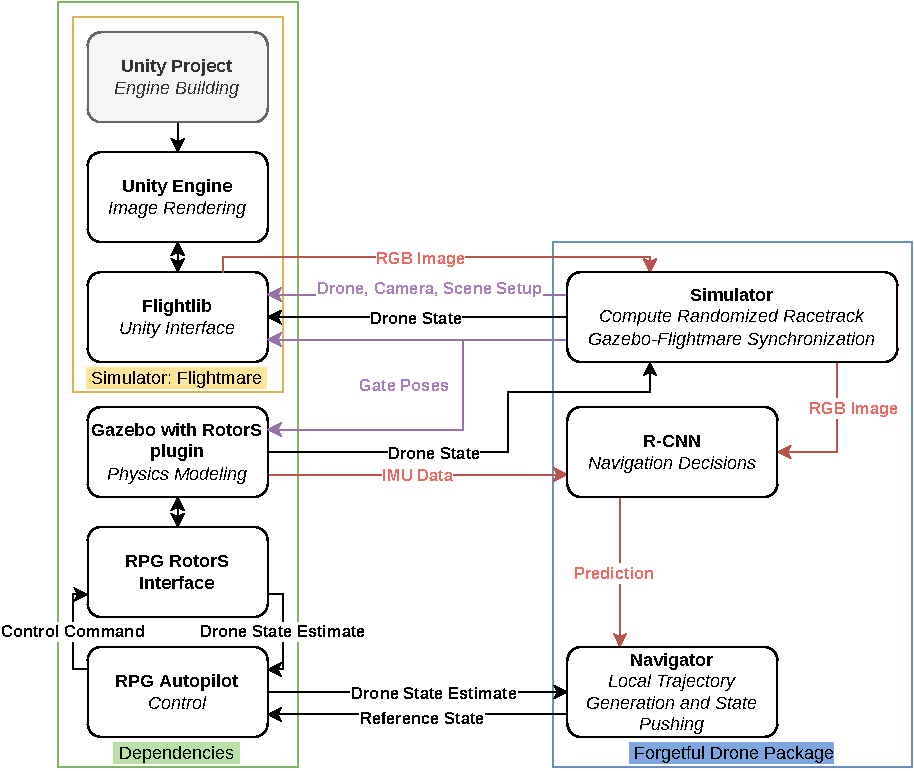
\includegraphics[width=1.0\textwidth]{figures/implementation_concept_network_testing.drawio.pdf}
%    \decoRule
    \caption[Implementation Concept, Network Testing]{\textbf{Implementation Concept, Network Testing:}
	In comparison with above, the R-CNN substitutes the expert system by making predicitons based on the
	RGB image and the IMU data. All ground truth drone states are replaced with state estimates, 
	except for the synchronization of Gazebo and Flightmare.}
    \label{fig:OverviewDiagram}
\end{figure}










